\begin{flushright} {\tiny {\color{gray} \tt fdm\_stokes2D.tex}} \end{flushright}
%~~~~~~~~~~~~~~~~~~~~~~~~~~~~~~~~~~~~~~~~~~~~~~~~~~~~~~~~~~~~~~~~~~~~~~~~~~~~~~~~~~~~~~~~~~~~~~~~~~

%---------------------------------------------------------
\subsection{Incompressible isoviscous 2D Stokes equations}


In the case of an incompressible and isoviscous flow, we can start  from 
the momentum equation
\begin{equation}
-\vec\nabla p + \vec\nabla \cdot {\bm \tau} + \rho \vec{g} = \vec{0}
\end{equation}
with 
\[
{\bm \tau} = 2 \eta \dot{\bm \varepsilon}(\vec\upnu)
\]
In 2D the strain rate tensor components are given by
\[
\dot{\varepsilon}_{xx}=\frac{\partial u}{\partial x}
\quad\quad\quad
\dot{\varepsilon}_{xy}=\frac{1}{2} \left( \frac{\partial u}{\partial y} + \frac{\partial v}{\partial x} \right)
\quad\quad\quad
\dot{\varepsilon}_{yy}=\frac{\partial v}{\partial y}
\]
In the end we obtain the following set of coupled PDEs for the three 
unknwons $u,v,p$:
\begin{eqnarray}
-\frac{\partial p}{\partial x}  
+ 2 \frac{\partial }{\partial x} \left(\eta \frac{\partial u}{\partial x}  \right) 
+\frac{\partial}{\partial y}\left(\eta (\frac{\partial u}{\partial y}+\frac{\partial v}{\partial x}) \right)
+  \rho g_x &=&0 \\
-\frac{\partial p}{\partial y}  
+ 2 \frac{\partial }{\partial y} \left(\eta \frac{\partial v}{\partial y}  \right) 
+\frac{\partial}{\partial x}\left(\eta (\frac{\partial u}{\partial y}+\frac{\partial v}{\partial x}) \right)
+  \rho g_y  &=& 0 \\
\frac{\partial u}{\partial x} + \frac{\partial v}{\partial y}  = 0 
\end{eqnarray}

Note that in their syllabus \textcite{beka} add the term $p/\lambda$ to the rhs
of the incompressibility equation: 
\begin{displayquote}
{\color{darkgray}
This is a ``trick'' called
the penalty method, which ensures that the system of equations does not become ill-
posed. For this to work, $\lambda$ should be sufficiently large 
($\sim 10^4$ or so), so that the condition
of incompressibility is approximately satisfied.}
\end{displayquote} 


Then, {\it if the viscosity is constant} the $x$-component of 
the momentum conservation equation
\[
-\frac{\partial p}{\partial x}  + 2\eta \frac{\partial \dot{\varepsilon}_{xx}}{\partial x} +  2\eta \frac{\partial \dot{\varepsilon}_{xy}}{\partial y}  + \rho g_x =0
\]
becomes
\[
-\frac{\partial p}{\partial x}  + 2\eta \frac{\partial^2 u}{\partial x^2} +  \eta 
\left( \frac{\partial^2 u}{\partial y^2 } + \frac{\partial^2 v}{\partial x \partial y} \right)  \rho g_x =0
\]
Using ${\vec \nabla} \cdot {\vec v} = 0$ to obtain $\frac{\partial u}{\partial x} =  - \frac{\partial v}{\partial y}  $ we arrive at 
\[
-\frac{\partial p}{\partial x}  + \eta \left( \frac{\partial^2 u}{\partial x^2} +  \frac{\partial^2 u}{\partial y^2 }  \right)
+ \rho g_x =0
\]
The same approach can be carried out for the $y$-component of the momentum conservation
equation and in the end
these are the three coupled equations we need to solve
\begin{eqnarray}
-\frac{\partial p}{\partial x}  
+ \eta \left( \frac{\partial^2 u}{\partial x^2} 
+ \frac{\partial^2 u}{\partial y^2 }  \right) + \rho g_x &=&0 \\
-\frac{\partial p}{\partial y}  
+ \eta \left( \frac{\partial^2 v}{\partial x^2} 
+ \frac{\partial^2 v}{\partial y^2 }  \right) + \rho g_y  &=& 0 \\
\frac{\partial u}{\partial x} + \frac{\partial v}{\partial y}  = 0 
\end{eqnarray}
Note that these must be supplemented by appropriate boundary conditions.

%------------------------------------
\subsection{The fully staggered grid}

Let us consider a 2D Cartesian domain of size $L_x \times L_y$.
It can be shown that the following layout of nodes is necessary 
if the FDM is to be successful\footnote{In other words
any attempt where $u$, $v$, $p$ would be on the corner nodes is doomed.}:
Note that in what follows we consider a mesh where all nodes are equidistant.
This is not a requirement of the method but it allows for more compact notations. 

\input{tikz/tikz_staggered2D}

There are:
\begin{itemize}
\item ${\tt ncellx}*{\tt ncelly}={\tt ncell}$ cells ($5*4$ above)
\item ${\tt ncell}$ pressure values ($20$ above)
\item ${\tt (ncellx+1)}*{\tt ncelly}$ $u$ unknowns ($6*4$ above) 
\item ${\tt ncell}*{\tt (ncelly+1)}$ $v$ unknowns ($5*5$ above) 
\item each cell is of size $h_x * h_y$ with $h_x=L_x/{\tt ncellx}$ 
and $h_y=L_y/{\tt ncelly}$.
\end{itemize}
In total there are (not taking boundary conditions into account)
$ndof$ unknowns with:
\[
ndof= {\tt ncellx}*{\tt ncelly} 
+ {\tt (ncellx+1)}*{\tt ncelly}
+ {\tt ncell}*{\tt (ncelly+1)}
\]
Note: the number of $u$ unknowns is not necessarily equal to the number of $v$
unknowns! This is nearly always the case with FEM. 

This means that once we have discretised the Stokes equations we will need
as many (i.e. $ndof$) equations in order to obtain a linear system with a solution.

%--------------------------------------------
\subsection{Solving the Laplacian formulation}

%...............................................
\subsubsection{momentum equation: $x$-component}

Let us zoom-in on a node which carries a $u$ unknown. 
We label it ${\tt ku}$. Its right ('east' or {\tt e})  neighbour is then ${\tt ku\_e}$,
its left ('west' or {\tt w}) neighbour is ${\tt ku\_w}$, 
its top ('north' or {\tt n}) neighbour is ${\tt ku\_n}$ and 
its bottom ('south' or {\tt s}) neighbour is ${\tt ku\_s}$.
Its nearest pressure nodes are ${\tt kp\_e}$ and ${\tt kp\_w}$, and the $v$ nodes
that surround it are ${\tt kv\_sw}$, ${\tt kv\_se}$, ${\tt kv\_ne}$ and ${\tt kv\_nw}$
as shown here:

\begin{flushright} {\tiny {\color{gray} (tikz\_staggered2D\_u.tex)}} \end{flushright}
%~~~~~~~~~~~~~~~~~~~~~~~~~~~~~~~~~~~~~~~~~~~~~~~~~~~~~~~~~~~~~~~~~~~~~~~~~~~~~~~~~~~~~~~~~~~~~~~~~~

\begin{center}
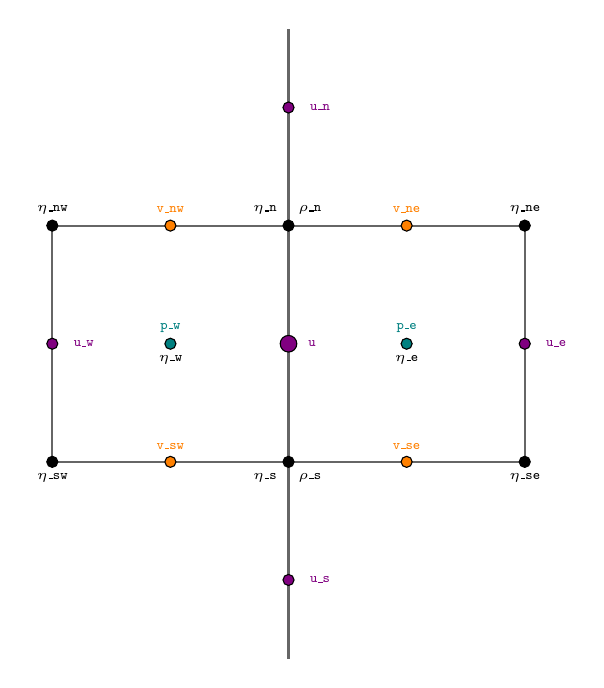
\begin{tikzpicture}
%\draw[fill=gray!23,gray!23](0,0) rectangle (8,9);
%\draw[step=0.5cm,gray,very thin] (0,0) grid (8,9); %background grid

\draw[thick,black!60] (1,3) -- (7,3) -- (7,6) -- (1,6) -- cycle ; 
\draw[thick,black!60] (4,0.5) -- (4,8.5)  ;   

%---------------------------------------------------
\node[] at (2.5,6.2) {\tiny \color{orange} \tt v\_nw};
\node[] at (2.5,3.2) {\tiny \color{orange} \tt v\_sw};
\node[] at (5.5,6.2) {\tiny \color{orange} \tt v\_ne};
\node[] at (5.5,3.2) {\tiny \color{orange} \tt v\_se};
\draw[black,fill=orange] (2.5,6)   circle (2pt);
\draw[black,fill=orange] (2.5,3)   circle (2pt);
\draw[black,fill=orange] (5.5,6)   circle (2pt);
\draw[black,fill=orange] (5.5,3)   circle (2pt);

%--------------------------------------------------
\draw[black,fill=violet] (4,1.5)   circle (2pt);
\draw[black,fill=violet] (4,4.5)   circle (3pt);
\draw[black,fill=violet] (4,7.5)   circle (2pt);
\draw[black,fill=violet] (1,4.5)   circle (2pt);
\draw[black,fill=violet] (7,4.5)   circle (2pt);
\node[] at (4.4,1.5) {\tiny \color{violet} \tt u\_s};
\node[] at (4.3,4.5) {\tiny \color{violet} \tt u};
\node[] at (4.4,7.5) {\tiny \color{violet} \tt u\_n};
\node[] at (1.4,4.5) {\tiny \color{violet} \tt u\_w};
\node[] at (7.4,4.5) {\tiny \color{violet} \tt u\_e};

\draw[black,fill=black] (1,3)   circle (2pt); 
\draw[black,fill=black] (4,3)   circle (2pt); 
\draw[black,fill=black] (7,3)   circle (2pt); 
\draw[black,fill=black] (1,6)   circle (2pt); 
\draw[black,fill=black] (4,6)   circle (2pt); 
\draw[black,fill=black] (7,6)   circle (2pt); 

%------------------------------------------------
\draw[black,fill=teal] (2.5,4.5)   circle (2pt);
\draw[black,fill=teal] (5.5,4.5)   circle (2pt);
\node[] at (2.5,4.7) {\tiny \color{teal} \tt p\_w};
\node[] at (5.5,4.7) {\tiny \color{teal} \tt p\_e};

\node[] at (4.27,2.8) {\tiny \tt $\rho$\_s};
\node[] at (4.27,6.2) {\tiny \tt $\rho$\_n};
\node[] at (2.5,4.3) {\tiny \tt $\eta$\_w};
\node[] at (5.5,4.3) {\tiny \tt $\eta$\_e};
\node[] at (3.7,2.8) {\tiny \tt $\eta$\_s};
\node[] at (3.7,6.2) {\tiny \tt $\eta$\_n};
\node[] at (7,6.2) {\tiny \tt $\eta$\_{ne}};
\node[] at (1,6.2) {\tiny \tt $\eta$\_{nw}};
\node[] at (7,2.8) {\tiny \tt $\eta$\_{se}};
\node[] at (1,2.8) {\tiny \tt $\eta$\_{sw}};
\end{tikzpicture}
\end{center}



We then have

\begin{eqnarray}
\left. -\frac{\partial p}{\partial x} \right|_{\tt ku}
&=& -\frac{{\tt p\_e}-{\tt p\_w}}{\tt hx}       \nn\\
\left. \eta \frac{\partial^2 u}{\partial x^2} \right|_{\tt ku}
&=& \eta \frac{{\tt u\_e} -2{\tt u}+{\tt u\_w}}{{\tt hx}^2}  \nn\\
\left. \eta \frac{\partial^2 u}{\partial y^2} \right|_{\tt ku}
&=& \eta \frac{{\tt u\_n}-2{\tt u}+{\tt u\_s}}{{\tt hy}^2}  \nn\\
\left. \rho g_x \right|_{\tt ku} 
&=& \frac{\rho_{\tt n} + \rho_{\tt s}}{2} g_x   \nn
\end{eqnarray}
For example, let us consider the $u$-node 9. Then the above stencils put together become:

\[
-\frac{p_{\tt 8}-p_{\tt 7}}{h_x}       
+
\eta \frac{u_{\tt 8} -2u_{\tt 9}+u_{\tt 10}}{h_x^2}  
+ 
\eta \frac{u_{\tt 3}-2u_{\tt 9}+u_{\tt 15}}{h_y^2}  
= -
\frac{\rho_{\tt 9} + \rho_{\tt 15}}{2} g_x  
\]

The lhs contains 7 unknowns: $p_{\tt 8}$, $p_{\tt 7}$, $u_{\tt 8}$,
$u_{\tt 9}$, $u_{\tt 10}$, $u_{\tt 3}$ and $u_{\tt 15}$.

{\color{red} is density on background mesh for sure?}


%...............................................
\subsubsection{momentum equation: $y$-component}

We now focus on a $v$ node with index ${\tt kv}$:

\begin{flushright} {\tiny {\color{gray} (tikz\_staggered2D\_v.tex)}} \end{flushright}
%~~~~~~~~~~~~~~~~~~~~~~~~~~~~~~~~~~~~~~~~~~~~~~~~~~~~~~~~~~~~~~~~~~~~~~~~~~~~~~~~~~~~~~~~~~~~~~~~~~



\begin{center}
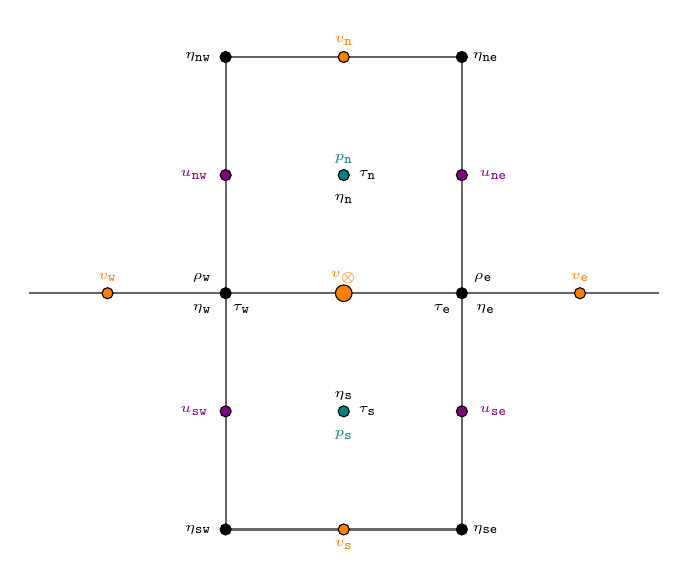
\begin{tikzpicture}
%\draw[fill=gray!23,gray!23](0,0) rectangle (9,8);
%\draw[step=0.5cm,gray,very thin] (0,0) grid (9,8); %background grid
\draw[thick,black!60] (3,1) -- (3,7) -- (6,7) -- (6,1) -- cycle ; 
\draw[thick,black!60] (0.5,4) -- (8.5,4)  ;   
%---------------------------------------------------
\node[] at (4.5,.8) {\tiny \color{orange} $v_{\tt s}$};
\node[] at (4.5,7.2) {\tiny \color{orange} $v_{\tt n}$};
\node[] at (4.5,4.2) {\tiny \color{orange} $v_\otimes$};
\node[] at (1.5,4.2) {\tiny \color{orange} $v_{\tt w}$};
\node[] at (7.5,4.2) {\tiny \color{orange} $v_{\tt e}$};
\draw[black,fill=orange] (4.5,1)   circle (2pt);
\draw[black,fill=orange] (4.5,4)   circle (3pt);
\draw[black,fill=orange] (4.5,7)   circle (2pt);
\draw[black,fill=orange] (1.5,4)   circle (2pt);
\draw[black,fill=orange] (7.5,4)   circle (2pt);
%--------------------------------------------------
\draw[black,fill=violet] (3,2.5)   circle (2pt);
\draw[black,fill=violet] (6,2.5)   circle (2pt);
\draw[black,fill=violet] (3,5.5)   circle (2pt);
\draw[black,fill=violet] (6,5.5)   circle (2pt);
\node[] at (2.6,2.5) {\tiny \color{violet} $u_{\tt sw}$};
\node[] at (6.4,2.5) {\tiny \color{violet} $u_{\tt se}$};
\node[] at (2.6,5.5) {\tiny \color{violet} $u_{\tt nw}$};
\node[] at (6.4,5.5) {\tiny \color{violet} $u_{\tt ne}$};
%-----------------------------------------------
\draw[black,fill=black] (3,1)   circle (2pt); 
\draw[black,fill=black] (3,4)   circle (2pt); 
\draw[black,fill=black] (3,7)   circle (2pt); 
\draw[black,fill=black] (6,1)   circle (2pt); 
\draw[black,fill=black] (6,4)   circle (2pt); 
\draw[black,fill=black] (6,7)   circle (2pt); 
%------------------------------------------------
\draw[black,fill=teal] (4.5,2.5)   circle (2pt);
\draw[black,fill=teal] (4.5,5.5)   circle (2pt);
\node[] at (4.5,2.2) {\tiny \color{teal} $p_{\tt s}$};
\node[] at (4.5,5.7) {\tiny \color{teal} $p_{\tt n}$};
%-----------------------------------------
\node[] at (6.27,4.2) {\tiny $\rho_{\tt e}$};
\node[] at (2.7,4.2) {\tiny $\rho_{\tt w}$};
\node[] at (4.5,5.2) {\tiny $\eta_{\tt n}$};
\node[] at (4.5,2.7) {\tiny $\eta_{\tt s}$};
\node[] at (6.3,1) {\tiny $\eta_{\tt se}$};
\node[] at (2.65,1) {\tiny $\eta_{\tt sw}$};
\node[] at (6.3,7) {\tiny $\eta_{\tt ne}$};
\node[] at (2.65,7) {\tiny $\eta_{\tt nw}$};
\node[] at (6.3,3.8) {\tiny $\eta_{\tt e}$};
\node[] at (2.7,3.8) {\tiny $\eta_{\tt w}$};

\node[] at (3.2,3.8) {\tiny $\tau_{\tt w}$};
\node[] at (5.75,3.8) {\tiny $\tau_{\tt e}$};
\node[] at (4.8,5.5) {\tiny $\tau_{\tt n}$};
\node[] at (4.8,2.5) {\tiny $\tau_{\tt s}$};


\end{tikzpicture}
\end{center}




\begin{eqnarray}
\left. -\frac{\partial p}{\partial y} \right|
&=& -\frac{{\tt p\_n}-{\tt p\_s}}{h_y}       \nn\\
\left. \eta \frac{\partial^2 v}{\partial x^2} \right|
&=& \eta \frac{{\tt v\_e} -2{\tt v}+{\tt v\_w}}{h_x^2}  \nn\\
\left. \eta \frac{\partial^2 v}{\partial y^2} \right|
&=& \eta \frac{{\tt v\_n} -2{\tt v}+{\tt v\_s}}{h_y^2}  \nn\\
\left. \rho g_y \right| 
&=& \frac{\rho_{\tt w} + \rho_{\tt e}}{2} g_y   \nn
\end{eqnarray}

For example, let us consider the $v$-node 13. Then the above stencils put together become:
\[
 -\frac{p_{\tt 13}-p_{\tt 8}}{h_y}       
+
\eta \frac{v_{\tt 14} -2v_{\tt 13}+v_{\tt 12}}{h_x^2} 
+
\eta \frac{v_{\tt 18} -2v_{\tt 13}+v_{\tt 8}}{h_y^2}  
= -
\frac{\rho_{\tt 15} + \rho_{\tt 16}}{2} g_y  
\]
The lhs contains 7 unknowns: $p_{\tt 13}$, $p_{\tt 8}$, $v_{\tt 14}$,
$v_{\tt 13}$, $v_{\tt 12}$, $v_{\tt 18}$ and $v_{\tt 8}$.



%...............................................
\subsubsection{Continuity equation}

In two dimensions the continuity equation
is 
\[
\vec\nabla \cdot \vec\upnu 
= 
\frac{\partial u}{\partial x} 
+
\frac{\partial v}{\partial y} 
=0
\]
We can isolate one cell:

\begin{flushright} {\tiny {\color{gray} (tikz\_staggered2D\_divv.tex)}} \end{flushright}
%~~~~~~~~~~~~~~~~~~~~~~~~~~~~~~~~~~~~~~~~~~~~~~~~~~~~~~~~~~~~~~~~~~~~~~~~~~~~~~~~~~~~~~~~~~~~~~~~~~


\begin{center}
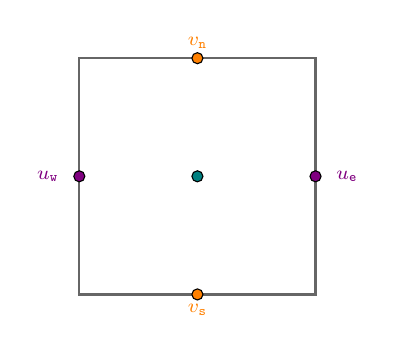
\begin{tikzpicture}
%\draw[fill=gray!23,gray!23](0,0) rectangle (5,5);
%\draw[step=0.5cm,gray,very thin] (0,0) grid (5,5); %background grid
\draw[thick,black!60] (1,1) -- (4,1) -- (4,4) -- (1,4) -- cycle ; 
\draw[black,fill=teal] (2.5,2.5)   circle (2pt);
%---------------------------------------------------
\node[] at (2.5,0.8) {\scriptsize \color{orange} $v_{\tt s}$};
\node[] at (2.5,4.2) {\scriptsize \color{orange} $v_{\tt n}$};
\draw[black,fill=orange] (2.5,1)   circle (2pt);
\draw[black,fill=orange] (2.5,4)   circle (2pt);
%---------------------------------------------------
\node[] at (0.6,2.5) {\scriptsize \color{violet} $u_{\tt w}$};
\node[] at (4.4,2.5) {\scriptsize \color{violet} $u_{\tt e}$};
\draw[black,fill=violet] (1,2.5)   circle (2pt);
\draw[black,fill=violet] (4,2.5)   circle (2pt);
\end{tikzpicture}
\end{center}






and discretise the equation above in its middle.
\[
\frac{u_{\tt ku\_e}-u_{\tt ku\_w}}{h_x} 
+
\frac{v_{\tt kv\_n}-v_{\tt kv\_s}}{h_y} 
=0
\]
For example, let us consider cell 14. Then the above stencil becomes:
\[
\frac{u_{\tt 17}-u_{\tt 16}}{h_x} + \frac{v_{\tt 19}-v_{\tt 14}}{h_y} =0
\]





%----------------------------------------------------------------
\subsubsection{Put it all together, let's be concrete}

Let us consider a $4\times 3$ mesh.
We have 12 cells, 15 $u$-nodes, 16 $v$-nodes and 12 $p$-nodes.
This mesh then counts $ndof=15+16+12=43$ unknowns.

\input{tikz/tikz_staggered2D_4x3}




Let us assume that we prescribe free slip on all sides.
Then we set $v_{\tt 1}=v_{\tt 2}=v_{\tt 3}=v_{\tt 4}=v_{\tt 13}=v_{\tt 14}=v_{\tt 15}=v_{\tt 16}=0$
and $u_{\tt 1}=u_{\tt 5}=u_{\tt 6}=u_{\tt 10}=u_{\tt 11} = u_{\tt 15}=0$.
This means that we need not discretise the momentum equation on these nodes.

IS IT CORRECT for free slip ??

Since we will need those in what follows, let us recall the forward, centered 
and backward (from left to right) formulation of a second-order derivative:
\[
f_i''=\frac{f_{i+2}-2f_{i+1}+f_i}{h^2}
\qquad
f_i''=\frac{f_{i+1}-2f_{i}+f_{i-1}}{h^2}
\qquad
f_i''=\frac{f_{i}-2f_{i-1}+f_{i-2}}{h^2}
\]

We must write the discretised $x$-momentum equation for the $u$ nodes nodes not on the 
boundary, so nodes 2,3,4,7,8,9,12,13,14.
However we must make a distinction between the nodes 2,3,4,12,13,14 and the nodes 7,8,9.
The latter ones have 4 $u$-node neighbours which allows us to discretise the 
second-order derivatives with a 
centered stencil. The former ones will require the use of forward (2,3,4) or backward (12,13,14) formulations.

\begin{itemize}
\item nodes 2,3,4
\begin{eqnarray}
-\frac{p_{\tt }-p_{\tt }}{h_x}       
+\eta \frac{u_{\tt } -2u_{\tt }+u_{\tt }}{h_x^2}  
+\eta \frac{u_{\tt }-2u_{\tt }+u_{\tt }}{h_y^2}  
&=& - \frac{\rho_{\tt } + \rho_{\tt }}{2} g_x  
\\
-\frac{p_{\tt }-p_{\tt }}{h_x}       
+\eta \frac{u_{\tt } -2u_{\tt }+u_{\tt }}{h_x^2}  
+\eta \frac{u_{\tt }-2u_{\tt }+u_{\tt }}{h_y^2}  
&=& - \frac{\rho_{\tt } + \rho_{\tt }}{2} g_x  
\\
-\frac{p_{\tt }-p_{\tt }}{h_x}       
+\eta \frac{u_{\tt } -2u_{\tt }+u_{\tt }}{h_x^2}  
+\eta \frac{u_{\tt }-2u_{\tt }+u_{\tt }}{h_y^2}  
&=& - \frac{\rho_{\tt } + \rho_{\tt }}{2} g_x  
\end{eqnarray}



\item nodes 7,8,9
\begin{eqnarray}
-\frac{p_{\tt 6}-p_{\tt 5}}{h_x}       
+\eta \frac{u_{\tt 6} -2u_{\tt 7}+u_{\tt 8}}{h_x^2}  
+\eta \frac{u_{\tt 2}-2u_{\tt 7}+u_{\tt 12}}{h_y^2}  
&=& - \frac{\rho_{\tt 7} + \rho_{\tt 12}}{2} g_x  
\\
-\frac{p_{\tt 7}-p_{\tt 6}}{h_x}       
+\eta \frac{u_{\tt 7} -2u_{\tt 8}+u_{\tt 9}}{h_x^2}  
+\eta \frac{u_{\tt 3}-2u_{\tt 8}+u_{\tt 13}}{h_y^2}  
&=& - \frac{\rho_{\tt 8} + \rho_{\tt 13}}{2} g_x  
\\
-\frac{p_{\tt 8}-p_{\tt 7}}{h_x}       
+\eta \frac{u_{\tt 8} -2u_{\tt 9}+u_{\tt 10}}{h_x^2}  
+\eta \frac{u_{\tt 4}-2u_{\tt 9}+u_{\tt 14}}{h_y^2}  
&=& - \frac{\rho_{\tt 9} + \rho_{\tt 14}}{2} g_x  
\end{eqnarray}


\item nodes 12,13,14

\begin{eqnarray}
-\frac{p_{\tt }-p_{\tt }}{h_x}       
+\eta \frac{u_{\tt } -2u_{\tt }+u_{\tt }}{h_x^2}  
+\eta \frac{u_{\tt }-2u_{\tt }+u_{\tt }}{h_y^2}  
&=& - \frac{\rho_{\tt } + \rho_{\tt }}{2} g_x  
\\
-\frac{p_{\tt }-p_{\tt }}{h_x}       
+\eta \frac{u_{\tt } -2u_{\tt }+u_{\tt }}{h_x^2}  
+\eta \frac{u_{\tt }-2u_{\tt }+u_{\tt }}{h_y^2}  
&=& - \frac{\rho_{\tt } + \rho_{\tt }}{2} g_x  
\\
-\frac{p_{\tt }-p_{\tt }}{h_x}       
+\eta \frac{u_{\tt } -2u_{\tt }+u_{\tt }}{h_x^2}  
+\eta \frac{u_{\tt }-2u_{\tt }+u_{\tt }}{h_y^2}  
&=& - \frac{\rho_{\tt } + \rho_{\tt }}{2} g_x  
\end{eqnarray}


\end{itemize}


Likewise, we must discretise the $y$-momentum equation on $v$-nodes 5,6,7,8,9,10,11,12.
Nodes 5,9 will require a forward scheme, nodes 8,12 will require a backward scheme, 
while a centered approach is suitable for nodes 6,7,10,11.

\begin{itemize}
\item nodes 5,9

\begin{eqnarray}
-\frac{p_{\tt }-p_{\tt }}{h_y}       
+ \eta \frac{v_{\tt } -2v_{\tt }+v_{\tt }}{h_x^2} 
+ \eta \frac{v_{\tt } -2v_{\tt }+v_{\tt }}{h_y^2}  
&=& - \frac{\rho_{\tt } + \rho_{\tt }}{2} g_y   
\\
-\frac{p_{\tt }-p_{\tt 2}}{h_y}       
+ \eta \frac{v_{\tt } -2v_{\tt }+v_{\tt }}{h_x^2} 
+ \eta \frac{v_{\tt } -2v_{\tt }+v_{\tt }}{h_y^2}  
&=& - \frac{\rho_{\tt } + \rho_{\tt }}{2} g_y   
\end{eqnarray}


\item nodes 8,12

\begin{eqnarray}
-\frac{p_{\tt }-p_{\tt }}{h_y}       
+ \eta \frac{v_{\tt } -2v_{\tt }+v_{\tt }}{h_x^2} 
+ \eta \frac{v_{\tt } -2v_{\tt }+v_{\tt }}{h_y^2}  
&=& - \frac{\rho_{\tt } + \rho_{\tt }}{2} g_y   
\\
-\frac{p_{\tt }-p_{\tt 2}}{h_y}       
+ \eta \frac{v_{\tt } -2v_{\tt }+v_{\tt }}{h_x^2} 
+ \eta \frac{v_{\tt } -2v_{\tt }+v_{\tt }}{h_y^2}  
&=& - \frac{\rho_{\tt } + \rho_{\tt }}{2} g_y   
\end{eqnarray}


\item nodes 6,7,10,11

\begin{eqnarray}
-\frac{p_{\tt }-p_{\tt }}{h_y}       
+ \eta \frac{v_{\tt } -2v_{\tt }+v_{\tt }}{h_x^2} 
+ \eta \frac{v_{\tt } -2v_{\tt }+v_{\tt }}{h_y^2}  
&=& - \frac{\rho_{\tt } + \rho_{\tt }}{2} g_y   
\\
-\frac{p_{\tt }-p_{\tt }}{h_y}       
+ \eta \frac{v_{\tt } -2v_{\tt }+v_{\tt }}{h_x^2} 
+ \eta \frac{v_{\tt } -2v_{\tt }+v_{\tt }}{h_y^2}  
&=& - \frac{\rho_{\tt } + \rho_{\tt }}{2} g_y   
\\
-\frac{p_{\tt }-p_{\tt }}{h_y}       
+ \eta \frac{v_{\tt } -2v_{\tt }+v_{\tt }}{h_x^2} 
+ \eta \frac{v_{\tt } -2v_{\tt }+v_{\tt }}{h_y^2}  
&=& - \frac{\rho_{\tt } + \rho_{\tt }}{2} g_y   
\\
-\frac{p_{\tt }-p_{\tt }}{h_y}       
+ \eta \frac{v_{\tt } -2v_{\tt }+v_{\tt }}{h_x^2} 
+ \eta \frac{v_{\tt } -2v_{\tt }+v_{\tt }}{h_y^2}  
&=& - \frac{\rho_{\tt } + \rho_{\tt }}{2} g_y   
\end{eqnarray}


\end{itemize}


The continuity equation in the middle of each cell yields 12 equations:
\begin{eqnarray}
\frac{u_{\tt 2}-u_{\tt 1}}{h_x} + \frac{v_{\tt 4}-v_{\tt 1}}{h_y} &=& 0 \\
\frac{u_{\tt 3}-u_{\tt 2}}{h_x} + \frac{v_{\tt 5}-v_{\tt 2}}{h_y} &=& 0 \\
\frac{u_{\tt 4}-u_{\tt 3}}{h_x} + \frac{v_{\tt 6}-v_{\tt 3}}{h_y} &=& 0 \\
\frac{u_{\tt 5}-u_{\tt 4}}{h_x} + \frac{v_{\tt 7}-v_{\tt 4}}{h_y} &=& 0 
\\
\frac{u_{\tt 7}-u_{\tt 6}}{h_x} + \frac{v_{\tt 9}-v_{\tt 5}}{h_y} &=& 0 \\
\frac{u_{\tt 8}-u_{\tt 7}}{h_x} + \frac{v_{\tt 10}-v_{\tt 6}}{h_y} &=& 0 \\
\frac{u_{\tt 9}-u_{\tt 8}}{h_x} + \frac{v_{\tt 11}-v_{\tt 7}}{h_y} &=& 0 \\
\frac{u_{\tt 10}-u_{\tt 9}}{h_x} + \frac{v_{\tt 12}-v_{\tt 8}}{h_y} &=& 0 
\\
\frac{u_{\tt 12}-u_{\tt 11}}{h_x} + \frac{v_{\tt 13}-v_{\tt 9}}{h_y} &=& 0 \\
\frac{u_{\tt 13}-u_{\tt 12}}{h_x} + \frac{v_{\tt 14}-v_{\tt 10}}{h_y} &=& 0 \\
\frac{u_{\tt 14}-u_{\tt 13}}{h_x} + \frac{v_{\tt 15}-v_{\tt 11}}{h_y} &=& 0 \\
\frac{u_{\tt 15}-u_{\tt 14}}{h_x} + \frac{v_{\tt 16}-v_{\tt 12}}{h_y} &=& 0 
\end{eqnarray}

Let us now create the vector $\vec{X}$ that is $ndof=23$ long:
\[
\vec{X}^T=(
u_{\tt 1},u_{\tt 2}, \dots , u_{\tt 15},
v_{\tt 1},v_{\tt 2}, \dots , v_{\tt 16},
p_{\tt 1},p_{\tt 2}, \dots, p_{\tt 12})
\]
We have 14 boundary conditions and 30 relationships between unknowns which we 
can write as a linear system.

\begin{landscape}
{\tiny
\[
\left(
\begin{array}{c|c|c|c|c|c|c|c|c|c|c|c|c|c|c|c|c|c|c|c|c|c|c|c|c|c|c|c|c|c|c|c|c|c|c|c|c|c|c|c|c|c|c}
1 & 2 & 3 & 4 & 5 & 6 & 7 & 8 & 9 &
10 & 11 &12 &13 &14 &15& 16& 17& 18& 19 &
20 &21 &22 &23 & 24 & 25 & 26 & 27 & 28 & 29 &
30 &21 &22 &23 & 24 & 25 & 26 & 27 & 28 & 29 &
40 & 41 & 42 & 43 \\
. & . & . & . & . & . & . & . & . & . & . & . & . & . & . & . & . & . & . & . & . & . & . & . & . & 
. & . & . & . & . & . & . & . & . & . & . & . & . & . & . & . & . & . \\
. & . & . & . & . & . & . & . & . & . & . & . & . & . & . & . & . & . & . & . & . & . & . & . & . & 
. & . & . & . & . & . & . & . & . & . & . & . & . & . & . & . & . & . \\
. & . & . & . & . & . & . & . & . & . & . & . & . & . & . & . & . & . & . & . & . & . & . & . & . & 
. & . & . & . & . & . & . & . & . & . & . & . & . & . & . & . & . & . \\
. & . & . & . & . & . & . & . & . & . & . & . & . & . & . & . & . & . & . & . & . & . & . & . & . & 
. & . & . & . & . & . & . & . & . & . & . & . & . & . & . & . & . & . \\
. & . & . & . & . & . & . & . & . & . & . & . & . & . & . & . & . & . & . & . & . & . & . & . & . & 
. & . & . & . & . & . & . & . & . & . & . & . & . & . & . & . & . & . \\
. & . & . & . & . & . & . & . & . & . & . & . & . & . & . & . & . & . & . & . & . & . & . & . & . & 
. & . & . & . & . & . & . & . & . & . & . & . & . & . & . & . & . & . \\
. & . & . & . & . & . & . & . & . & . & . & . & . & . & . & . & . & . & . & . & . & . & . & . & . & 
. & . & . & . & . & . & . & . & . & . & . & . & . & . & . & . & . & . \\
. & . & . & . & . & . & . & . & . & . & . & . & . & . & . & . & . & . & . & . & . & . & . & . & . & 
. & . & . & . & . & . & . & . & . & . & . & . & . & . & . & . & . & . \\
. & . & . & . & . & . & . & . & . & . & . & . & . & . & . & . & . & . & . & . & . & . & . & . & . & 
. & . & . & . & . & . & . & . & . & . & . & . & . & . & . & . & . & . \\
. & . & . & . & . & . & . & . & . & . & . & . & . & . & . & . & . & . & . & . & . & . & . & . & . & 
. & . & . & . & . & . & . & . & . & . & . & . & . & . & . & . & . & . \\
\hline
. & . & . & . & . & . & . & . & . & . & . & . & . & . & . & . & . & . & . & . & . & . & . & . & . & 
. & . & . & . & . & . & . & . & . & . & . & . & . & . & . & . & . & . \\
. & . & . & . & . & . & . & . & . & . & . & . & . & . & . & . & . & . & . & . & . & . & . & . & . & 
. & . & . & . & . & . & . & . & . & . & . & . & . & . & . & . & . & . \\
. & . & . & . & . & . & . & . & . & . & . & . & . & . & . & . & . & . & . & . & . & . & . & . & . & 
. & . & . & . & . & . & . & . & . & . & . & . & . & . & . & . & . & . \\
. & . & . & . & . & . & . & . & . & . & . & . & . & . & . & . & . & . & . & . & . & . & . & . & . & 
. & . & . & . & . & . & . & . & . & . & . & . & . & . & . & . & . & . \\
. & . & . & . & . & . & . & . & . & . & . & . & . & . & . & . & . & . & . & . & . & . & . & . & . & 
. & . & . & . & . & . & . & . & . & . & . & . & . & . & . & . & . & . \\
. & . & . & . & . & . & . & . & . & . & . & . & . & . & . & . & . & . & . & . & . & . & . & . & . & 
. & . & . & . & . & . & . & . & . & . & . & . & . & . & . & . & . & . \\
. & . & . & . & . & . & . & . & . & . & . & . & . & . & . & . & . & . & . & . & . & . & . & . & . & 
. & . & . & . & . & . & . & . & . & . & . & . & . & . & . & . & . & . \\
. & . & . & . & . & . & . & . & . & . & . & . & . & . & . & . & . & . & . & . & . & . & . & . & . & 
. & . & . & . & . & . & . & . & . & . & . & . & . & . & . & . & . & . \\
. & . & . & . & . & . & . & . & . & . & . & . & . & . & . & . & . & . & . & . & . & . & . & . & . & 
. & . & . & . & . & . & . & . & . & . & . & . & . & . & . & . & . & . \\
. & . & . & . & . & . & . & . & . & . & . & . & . & . & . & . & . & . & . & . & . & . & . & . & . & 
. & . & . & . & . & . & . & . & . & . & . & . & . & . & . & . & . & . \\
\hline
. & . & . & . & . & . & . & . & . & . & . & . & . & . & . & . & . & . & . & . & . & . & . & . & . & 
. & . & . & . & . & . & . & . & . & . & . & . & . & . & . & . & . & . \\
. & . & . & . & . & . & . & . & . & . & . & . & . & . & . & . & . & . & . & . & . & . & . & . & . & 
. & . & . & . & . & . & . & . & . & . & . & . & . & . & . & . & . & . \\
. & . & . & . & . & . & . & . & . & . & . & . & . & . & . & . & . & . & . & . & . & . & . & . & . & 
. & . & . & . & . & . & . & . & . & . & . & . & . & . & . & . & . & . \\
. & . & . & . & . & . & . & . & . & . & . & . & . & . & . & . & . & . & . & . & . & . & . & . & . & 
. & . & . & . & . & . & . & . & . & . & . & . & . & . & . & . & . & . \\
. & . & . & . & . & . & . & . & . & . & . & . & . & . & . & . & . & . & . & . & . & . & . & . & . & 
. & . & . & . & . & . & . & . & . & . & . & . & . & . & . & . & . & . \\
. & . & . & . & . & . & . & . & . & . & . & . & . & . & . & . & . & . & . & . & . & . & . & . & . & 
. & . & . & . & . & . & . & . & . & . & . & . & . & . & . & . & . & . \\
. & . & . & . & . & . & . & . & . & . & . & . & . & . & . & . & . & . & . & . & . & . & . & . & . & 
. & . & . & . & . & . & . & . & . & . & . & . & . & . & . & . & . & . \\
. & . & . & . & . & . & . & . & . & . & . & . & . & . & . & . & . & . & . & . & . & . & . & . & . & 
. & . & . & . & . & . & . & . & . & . & . & . & . & . & . & . & . & . \\
. & . & . & . & . & . & . & . & . & . & . & . & . & . & . & . & . & . & . & . & . & . & . & . & . & 
. & . & . & . & . & . & . & . & . & . & . & . & . & . & . & . & . & . \\
. & . & . & . & . & . & . & . & . & . & . & . & . & . & . & . & . & . & . & . & . & . & . & . & . & 
. & . & . & . & . & . & . & . & . & . & . & . & . & . & . & . & . & . \\
\hline
. & . & . & . & . & . & . & . & . & . & . & . & . & . & . & . & . & . & . & . & . & . & . & . & . & 
. & . & . & . & . & . & . & . & . & . & . & . & . & . & . & . & . & . \\
. & . & . & . & . & . & . & . & . & . & . & . & . & . & . & . & . & . & . & . & . & . & . & . & . & 
. & . & . & . & . & . & . & . & . & . & . & . & . & . & . & . & . & . \\
. & . & . & . & . & . & . & . & . & . & . & . & . & . & . & . & . & . & . & . & . & . & . & . & . & 
. & . & . & . & . & . & . & . & . & . & . & . & . & . & . & . & . & . \\
. & . & . & . & . & . & . & . & . & . & . & . & . & . & . & . & . & . & . & . & . & . & . & . & . & 
. & . & . & . & . & . & . & . & . & . & . & . & . & . & . & . & . & . \\
. & . & . & . & . & . & . & . & . & . & . & . & . & . & . & . & . & . & . & . & . & . & . & . & . & 
. & . & . & . & . & . & . & . & . & . & . & . & . & . & . & . & . & . \\
. & . & . & . & . & . & . & . & . & . & . & . & . & . & . & . & . & . & . & . & . & . & . & . & . & 
. & . & . & . & . & . & . & . & . & . & . & . & . & . & . & . & . & . \\
. & . & . & . & . & . & . & . & . & . & . & . & . & . & . & . & . & . & . & . & . & . & . & . & . & 
. & . & . & . & . & . & . & . & . & . & . & . & . & . & . & . & . & . \\
. & . & . & . & . & . & . & . & . & . & . & . & . & . & . & . & . & . & . & . & . & . & . & . & . & 
. & . & . & . & . & . & . & . & . & . & . & . & . & . & . & . & . & . \\
. & . & . & . & . & . & . & . & . & . & . & . & . & . & . & . & . & . & . & . & . & . & . & . & . & 
. & . & . & . & . & . & . & . & . & . & . & . & . & . & . & . & . & . \\
. & . & . & . & . & . & . & . & . & . & . & . & . & . & . & . & . & . & . & . & . & . & . & . & . & 
. & . & . & . & . & . & . & . & . & . & . & . & . & . & . & . & . & . \\
\hline
. & . & . & . & . & . & . & . & . & . & . & . & . & . & . & . & . & . & . & . & . & . & . & . & . & 
. & . & . & . & . & . & . & . & . & . & . & . & . & . & . & . & . & . \\
. & . & . & . & . & . & . & . & . & . & . & . & . & . & . & . & . & . & . & . & . & . & . & . & . & 
. & . & . & . & . & . & . & . & . & . & . & . & . & . & . & . & . & . \\
. & . & . & . & . & . & . & . & . & . & . & . & . & . & . & . & . & . & . & . & . & . & . & . & . & 
. & . & . & . & . & . & . & . & . & . & . & . & . & . & . & . & . & . 
\end{array}
\right)
%\cdot
%\vec{X}=
%\left(
%\begin{array}{c}
%0 \\ . \\ . \\ 0 \\ 0 \\ . \\ . \\ 0 \\
%X \\
%0 \\ 0 \\ 0 \\ 0\\ 0 \\ 0
%\end{array}
%\right)
\]
}
\end{landscape}

In the end the matrix structure is 
\[
\left(
\begin{array}{ccc}
\K_{xx} & 0 & \G_x \\
0 & \K_{yy} & \G_y \\
\G_x^T & \G_y^T & 0
\end{array}
\right)
\]
with $\K_{xx}$ of size $N_u \times N_u$, etc ....

%...................................................
\subsubsection{A different way to deal with b.c.}

See fig 4.19 of beka. 
Within the purple domain, the
finite difference scheme for center points can be applied. At the boundaries, we have to apply a
special finite difference scheme which employ fictious boundary nodes.






%---------------------------------------------------
\subsection{generic approach}

\subsubsection{momentum equation: $x$-component}

\begin{center}
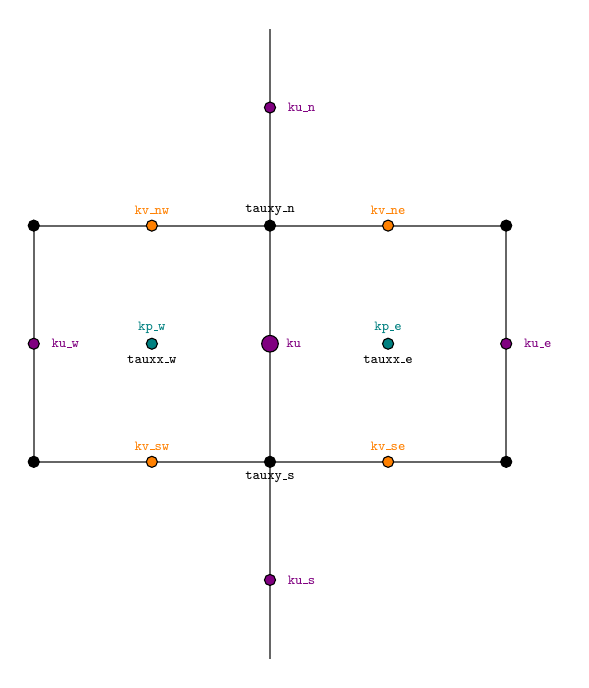
\begin{tikzpicture}
%\draw[fill=gray!23,gray!23](0,0) rectangle (8,9);
%\draw[step=0.5cm,gray,very thin] (0,0) grid (8,9); %background grid

\draw[thick,black!60] (1,3) -- (7,3) -- (7,6) -- (1,6) -- cycle ; 
\draw[thick,black!60] (4,0.5) -- (4,8.5)  ; 

%---------------------------------------------------
\node[] at (2.5,6.2) {\tiny \color{orange} \tt kv\_nw};
\node[] at (2.5,3.2) {\tiny \color{orange} \tt kv\_sw};
\node[] at (5.5,6.2) {\tiny \color{orange} \tt kv\_ne};
\node[] at (5.5,3.2) {\tiny \color{orange} \tt kv\_se};
\draw[black,fill=orange] (2.5,6)   circle (2pt);
\draw[black,fill=orange] (2.5,3)   circle (2pt);
\draw[black,fill=orange] (5.5,6)   circle (2pt);
\draw[black,fill=orange] (5.5,3)   circle (2pt);

%--------------------------------------------------
\draw[black,fill=violet] (4,1.5)   circle (2pt);
\draw[black,fill=violet] (4,4.5)   circle (3pt);
\draw[black,fill=violet] (4,7.5)   circle (2pt);
\draw[black,fill=violet] (1,4.5)   circle (2pt);
\draw[black,fill=violet] (7,4.5)   circle (2pt);
\node[] at (4.4,1.5) {\tiny \color{violet} \tt ku\_s};
\node[] at (4.3,4.5) {\tiny \color{violet} \tt ku};
\node[] at (4.4,7.5) {\tiny \color{violet} \tt ku\_n};
\node[] at (1.4,4.5) {\tiny \color{violet} \tt ku\_w};
\node[] at (7.4,4.5) {\tiny \color{violet} \tt ku\_e};

\draw[black,fill=black] (1,3)   circle (2pt); 
\draw[black,fill=black] (4,3)   circle (2pt); 
\draw[black,fill=black] (7,3)   circle (2pt); 
\draw[black,fill=black] (1,6)   circle (2pt); 
\draw[black,fill=black] (4,6)   circle (2pt); 
\draw[black,fill=black] (7,6)   circle (2pt); 


%------------------------------------------------
\draw[black,fill=teal] (2.5,4.5)   circle (2pt);
\draw[black,fill=teal] (5.5,4.5)   circle (2pt);
\node[] at (2.5,4.7) {\tiny \color{teal} \tt kp\_w};
\node[] at (5.5,4.7) {\tiny \color{teal} \tt kp\_e};

\node[] at (5.5,4.3) {\tiny \tt tauxx\_e};
\node[] at (2.5,4.3) {\tiny \tt tauxx\_w};
\node[] at (4,2.8) {\tiny \tt tauxy\_s};
\node[] at (4,6.2) {\tiny \tt tauxy\_n};

\end{tikzpicture}
\end{center}


The $x$-component of the momentum equation is given by
\[
-\frac{\partial p}{\partial x} + 
\frac{\partial \tau_{xx}}{\partial x} +
\frac{\partial \tau_{xy}}{\partial y} + \rho g_x = 0
\]


We have
\begin{eqnarray}
\left. -\frac{\partial p}{\partial x} \right|_{ku} 
&=& \frac{p_{kp\_e}-p_{kp\_w}}{h_x} \nn\\
\left. \frac{\partial \tau_{xx}}{\partial x}  \right|_{ku} 
&=&
\frac{\tau_{xx}|_e - \tau_{xx}|_w}{h_x} \nn\\
\left. \frac{\partial \tau_{xy}}{\partial y}  \right|_{ku} 
&=&
\frac{\tau_{xy}|_n - \tau_{xy}|_s}{h_y}
\end{eqnarray}
Since
\begin{eqnarray}
\tau_{xx}|_e &=& 2 \eta_e \dot\varepsilon_{xx}|_e \\
\tau_{xx}|_w &=& 2 \eta_w \dot\varepsilon_{xx}|_w \\
\tau_{xy}|_n &=& 2 \eta_e \dot\varepsilon_{xy}|_n \\
\tau_{xy}|_s &=& 2 \eta_w \dot\varepsilon_{xy}|_s
\end{eqnarray}





\begin{eqnarray}
\dot\varepsilon_{xx}|_e 
&=& \left.\frac{\partial u}{\partial x} \right|_e
 =\frac{u_{ku\_e}-u_{ku}  }{h_x}
\nn\\
\dot\varepsilon_{xx}|_w 
&=& \left.\frac{\partial u}{\partial x} \right|_w
=\frac{u_{ku}-u_{ku\_w}  }{h_x}
\nn\\
\dot\varepsilon_{xy}|_n &=&  
\frac12 \left( 
\left.\frac{\partial u}{\partial y} \right|_n
+ 
\left.\frac{\partial v}{\partial x} \right|_n \right)
=\left(
\frac{u_{ku\_n}-u_{ku}  }{h_y}
+
\frac{v_{kv\_ne}-v_{kv\_nw}  }{h_x}
\right)
\nn\\
\dot\varepsilon_{xy}|_s &=& 
\frac12 \left( 
\left.\frac{\partial u}{\partial y} \right|_s
+ 
\left.\frac{\partial v}{\partial x} \right|_s \right)
=\left(
\frac{u_{ku}-u_{ku\_s}  }{h_y}
+
\frac{v_{kv\_se}-v_{kv\_sw}  }{h_x}
\right)
\end{eqnarray}








then
\[
\left. \frac{\partial \tau_{xx}}{\partial x}  \right|_{ku} 
=
2 \eta_e \frac{u_{ku\_e}-u_{ku}  }{h_x^2}
-
2 \eta_w \frac{u_{ku}-u_{ku\_w}  }{h_x^2}
\]

\[
\left. \frac{\partial \tau_{xy}}{\partial y}  \right|_{ku} 
=
 \eta_n \left(
\frac{u_{ku\_n}-u_{ku}  }{h_y^2}
+
\frac{v_{kv\_ne}-v_{kv\_nw}  }{h_xh_y}
\right)
-
 \eta_s \left(
\frac{u_{ku}-u_{ku\_s}  }{h_y^2}
+
\frac{v_{kv\_se}-v_{kv\_sw}  }{h_xh_y}
\right)
\]




\subsubsection{momentum equation: $y$-component}

\begin{center}
\begin{tikzpicture}
%\draw[fill=gray!23,gray!23](0,0) rectangle (9,8);
%\draw[step=0.5cm,gray,very thin] (0,0) grid (9,8); %background grid
\draw[thick,black!60] (3,1) -- (3,7) -- (6,7) -- (6,1) -- cycle ; 
\draw[thick,black!60] (0.5,4) -- (8.5,4)  ; 
%---------------------------------------------------
\node[] at (4.5,.8) {\tiny \color{orange} \tt kv\_s};
\node[] at (4.5,7.2) {\tiny \color{orange} \tt kv\_n};
\node[] at (4.5,4.2) {\tiny \color{orange} \tt kv};
\node[] at (1.5,4.2) {\tiny \color{orange} \tt kv\_w};
\node[] at (7.5,4.2) {\tiny \color{orange} \tt kv\_e};
\draw[black,fill=orange] (4.5,1)   circle (2pt);
\draw[black,fill=orange] (4.5,4)   circle (2pt);
\draw[black,fill=orange] (4.5,7)   circle (2pt);
\draw[black,fill=orange] (1.5,4)   circle (2pt);
\draw[black,fill=orange] (7.5,4)   circle (2pt);
%--------------------------------------------------
\draw[black,fill=violet] (3,2.5)   circle (2pt);
\draw[black,fill=violet] (6,2.5)   circle (2pt);
\draw[black,fill=violet] (3,5.5)   circle (2pt);
\draw[black,fill=violet] (6,5.5)   circle (2pt);
\node[] at (2.5,2.5) {\tiny \color{violet} \tt ku\_sw};
\node[] at (6.5,2.5) {\tiny \color{violet} \tt ku\_se};
\node[] at (2.5,5.5) {\tiny \color{violet} \tt ku\_nw};
\node[] at (6.5,5.5) {\tiny \color{violet} \tt ku\_ne};
%-----------------------------------------------
\draw[black,fill=black] (3,1)   circle (2pt); 
\draw[black,fill=black] (3,4)   circle (2pt); 
\draw[black,fill=black] (3,7)   circle (2pt); 
\draw[black,fill=black] (6,1)   circle (2pt); 
\draw[black,fill=black] (6,4)   circle (2pt); 
\draw[black,fill=black] (6,7)   circle (2pt); 
%------------------------------------------------
\draw[black,fill=teal] (4.5,2.5)   circle (2pt);
\draw[black,fill=teal] (4.5,5.5)   circle (2pt);
\node[] at (4.5,2.2) {\tiny \color{teal} \tt kp\_s};
\node[] at (4.5,5.7) {\tiny \color{teal} \tt kp\_n};
%-----------------------------------------
\node[] at (6,4.3) {\tiny \tt tauxy\_e};
\node[] at (3,4.3) {\tiny \tt tauxy\_w};
\node[] at (4.5,2.8) {\tiny \tt tauyy\_s};
\node[] at (4.5,5.2) {\tiny \tt tauyy\_n};
\end{tikzpicture}
\end{center}


The $y$-component of the momentum equation is given by
\[
-\frac{\partial p}{\partial y} + 
\frac{\partial \tau_{xy}}{\partial x} +
\frac{\partial \tau_{yy}}{\partial y} + \rho g_y = 0
\]


We have
\begin{eqnarray}
\left. -\frac{\partial p}{\partial y} \right|_{kv} 
&=& 
-\frac{p_{kp\_n}-p_{kp\_s}}{h_y}
\\
\left. \frac{\partial \tau_{xy}}{\partial x}  \right|_{kv} 
&=&
\frac{\tau_{xy}|_e - \tau_{xy}|_w}{h_x}
\\
\left. \frac{\partial \tau_{yy}}{\partial y}  \right|_{kv} 
&=&
\frac{\tau_{yy}|_n - \tau_{yy}|_s}{h_y}
\end{eqnarray}
Since
\begin{eqnarray}
\tau_{xy}|_e &=& 2 \eta_e \dot\varepsilon_{xy}|_e \\
\tau_{xy}|_w &=& 2 \eta_w \dot\varepsilon_{xy}|_w \\
\tau_{yy}|_n &=& 2 \eta_e \dot\varepsilon_{yy}|_n \\
\tau_{yy}|_s &=& 2 \eta_w \dot\varepsilon_{yy}|_s
\end{eqnarray}
and 
\begin{eqnarray}
\dot\varepsilon_{xy}|_e 
&=& \frac12 \left( 
\left.\frac{\partial u}{\partial y} \right|_e
+ 
\left.\frac{\partial v}{\partial x} \right|_e \right)
=
\frac12 \left(
\frac{u_{ku\_ne}-u_{ku\_se}}{h_y}
+
\frac{v_{kv\_e}-v_{kv}}{h_x}
\right) 
\nn\\
\dot\varepsilon_{xy}|_w 
&=& \frac12 \left( 
\left.\frac{\partial u}{\partial y} \right|_w
+ 
\left.\frac{\partial v}{\partial x} \right|_w \right)
=
\frac12 \left(
\frac{u_{ku\_nw}-u_{ku\_sw}}{h_y}
+
\frac{v_{kv}-v_{kv\_w}}{h_x}
\right) 
\nn\\
\dot\varepsilon_{yy}|_n
&=& 
\left. \frac{\partial v}{\partial y}\right|_n = \frac{v_{kv\_n}-v_{kv} }{h_y} \nn\\
\dot\varepsilon_{yy}|_s
&=& 
\left. \frac{\partial v}{\partial y}\right|_s = \frac{v_{kv}-v_{kv\_s} }{h_y} 
\end{eqnarray}
In the end the full discretised equation writes

\[
\left. -\frac{\partial p}{\partial y} \right|_{kv} 
+
\left. \frac{\partial \tau_{xy}}{\partial x}  \right|_{kv} 
+
\left. \frac{\partial \tau_{yy}}{\partial y}  \right|_{kv} 
+ \rho_{kv} g_y = 0
\]
or, using all the equations above in turn:
\[
-\frac{p_{kp\_n}-p_{kp\_s}}{h_y}
+
\frac{\tau_{xy}|_e - \tau_{xy}|_w}{h_x}
+
\frac{\tau_{yy}|_n - \tau_{yy}|_s}{h_y} 
+ \rho_{kv} g_y = 0
\]
\[
-\frac{p_{kp\_n}-p_{kp\_s}}{h_y}
+ \frac{1}{h_x} \tau_{xy}|_e -\frac{1}{h_x} \tau_{xy}|_w
+ \frac{1 }{h_y} \tau_{yy}|_n -\frac{1}{h_y} \tau_{yy}|_s
+ \rho_{kv} g_y = 0
\]
\[
-\frac{p_{kp\_n}-p_{kp\_s}}{h_y}
+ \frac{2 \eta_e}{h_x}  \dot\varepsilon_{xy}|_e 
-\frac{2 \eta_w}{h_x}  \dot\varepsilon_{xy}|_w
+ \frac{2 \eta_e }{h_y}  \dot\varepsilon_{yy}|_n \\
-\frac{2 \eta_s}{h_y}  \dot\varepsilon_{yy}|_s \\
+ \rho_{kv} g_y = 0
\]




